%-- Template based off http://www.latextemplates.com/template/structured-general-purpose-assignment.

%%%%%%%%%%%%%%%%%%%%%%%%%%%%%%%%%%%%%%%%%
% Structured General Purpose Assignment
% LaTeX Template
%
% This template has been downloaded from:
% http://www.latextemplates.com
%
% Original author:
% Ted Pavlic (http://www.tedpavlic.com)
%
% Note:
% The \lipsum[#] commands throughout this template generate dummy text
% to fill the template out. These commands should all be removed when 
% writing assignment content.
%
%%%%%%%%%%%%%%%%%%%%%%%%%%%%%%%%%%%%%%%%%

%----------------------------------------------------------------------------------------
%	PACKAGES AND OTHER DOCUMENT CONFIGURATIONS
%----------------------------------------------------------------------------------------

\documentclass{article}

\usepackage{fancyhdr} % Required for custom headers
\usepackage{lastpage} % Required to determine the last page for the footer
\usepackage{extramarks} % Required for headers and footers
\usepackage{graphicx} % Required for including pictures
\usepackage{biblatex}
\usepackage{caption}


\bibliography{main.bib}
\graphicspath{ {images/} }

% Margins
\topmargin=-0.45in
\evensidemargin=0in
\oddsidemargin=0in
\textwidth=6.5in
\textheight=9.0in
\headsep=0.25in 

\linespread{1.1} % Line spacing

% Set up the header and footer
\pagestyle{fancy}
\lhead{\hmwkTitle} % Top left header
\chead{\hmwkShortCode} % Top center header
\rhead{\hmwkAuthorName} % Top right header
\lfoot{\lastxmark} % Bottom left footer
\cfoot{} % Bottom center footer
\rfoot{Page\ \thepage\ of\ \pageref{LastPage}} % Bottom right footer
\renewcommand\headrulewidth{0.4pt} % Size of the header rule
\renewcommand\footrulewidth{0.4pt} % Size of the footer rule

\setlength\parindent{0pt} % Removes all indentation from paragraphs

%----------------------------------------------------------------------------------------
%	DOCUMENT STRUCTURE COMMANDS
%	Skip this unless you know what you're doing
%----------------------------------------------------------------------------------------

% Header and footer for when a page split occurs within a problem environment
\newcommand{\enterProblemHeader}[1]{
\nobreak\extramarks{#1}{#1 continued on next page\ldots}\nobreak
\nobreak\extramarks{#1 (continued)}{#1 continued on next page\ldots}\nobreak
}

% Header and footer for when a page split occurs between problem environments
\newcommand{\exitProblemHeader}[1]{
\nobreak\extramarks{#1 (continued)}{#1 continued on next page\ldots}\nobreak
\nobreak\extramarks{#1}{}\nobreak
}

\setcounter{secnumdepth}{0} % Removes default section numbers
\newcounter{homeworkProblemCounter} % Creates a counter to keep track of the number of problems

\newcommand{\homeworkProblemName}{}
\newenvironment{homeworkProblem}[1][Problem \arabic{homeworkProblemCounter}]{ % Makes a new environment called homeworkProblem which takes 1 argument (custom name) but the default is "Problem #"
\stepcounter{homeworkProblemCounter} % Increase counter for number of problems
\renewcommand{\homeworkProblemName}{#1} % Assign \homeworkProblemName the name of the problem
\section{\homeworkProblemName} % Make a section in the document with the custom problem count
\enterProblemHeader{\homeworkProblemName} % Header and footer within the environment
}{
\exitProblemHeader{\homeworkProblemName} % Header and footer after the environment
}

\newcommand{\problemAnswer}[1]{ % Defines the problem answer command with the content as the only argument
\noindent\framebox[\columnwidth][c]{\begin{minipage}{0.98\columnwidth}#1\end{minipage}} % Makes the box around the problem answer and puts the content inside
}

\newcommand{\homeworkSectionName}{}
\newenvironment{homeworkSection}[1]{ % New environment for sections within homework problems, takes 1 argument - the name of the section
\renewcommand{\homeworkSectionName}{#1} % Assign \homeworkSectionName to the name of the section from the environment argument
\subsection{\homeworkSectionName} % Make a subsection with the custom name of the subsection
\enterProblemHeader{\homeworkProblemName\ [\homeworkSectionName]} % Header and footer within the environment
}{
\enterProblemHeader{\homeworkProblemName} % Header and footer after the environment
}
   
%----------------------------------------------------------------------------------------
%	NAME AND CLASS SECTION
%----------------------------------------------------------------------------------------

\newcommand{\hmwkTitle}{Enhancing the CS-Alumni Application} % Assignment title
\newcommand{\hmwkDueDate}{Monday,\ Decemeber\ 8,\ 2014} % Due date
\newcommand{\hmwkShortCode}{SE31520}
\newcommand{\hmwkClass}{Developing Internet-Based Applications} % Course/class
\newcommand{\hmwkClassTime}{4pm} % Class/lecture time
\newcommand{\hmwkAuthorName}{Thomas Mark Rosier (THR2)} % Your name
\newcommand{\hmwkStudentId}{110113188} % Student ID

%----------------------------------------------------------------------------------------
%	TITLE PAGE
%----------------------------------------------------------------------------------------

\title{
\vspace{2in}
\textmd{\textbf{\hmwkShortCode\\ \hmwkClass}}\\
\normalsize
\vspace{0.1in}
\textbf{\hmwkTitle}\\
\vspace{0.1in}
\small{Submission\ Due\ \hmwkClassTime\ \hmwkDueDate}\\
\vspace{3in}
}

\author{
\textbf{\hmwkAuthorName}\\
\hmwkStudentId
}
\date{} % Insert date here if you want it to appear below your name

%----------------------------------------------------------------------------------------

\begin{document}

\maketitle

%----------------------------------------------------------------------------------------
%	TABLE OF CONTENTS
%----------------------------------------------------------------------------------------

%\setcounter{tocdepth}{1} % Uncomment this line if you don't want subsections listed in the ToC

\newpage
\tableofcontents
\newpage


\nocite{bara:2013:online}
\nocite{saa:2013:online}

%-- Document Summary.
\section{Document Summary}

%-- Application Design.
\section{Application Design}

\subsection{CS-Alumni Chrome Browser Extension}

\subsubsection{Rational}

\subsubsection{Module Diagrams}

\subsubsection{Program Operation}

\begin{figure}[!htbp]
\centering
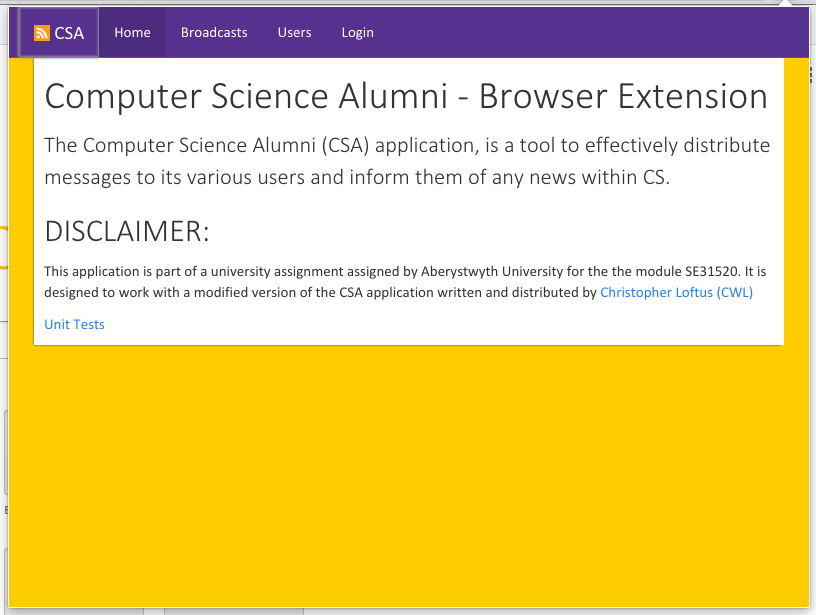
\includegraphics[width=0.8\textwidth]{homepage}
\caption{The screenshot above is the landing screen for the browser extension.}
\end{figure}

\begin{figure}[!htbp]
\centering
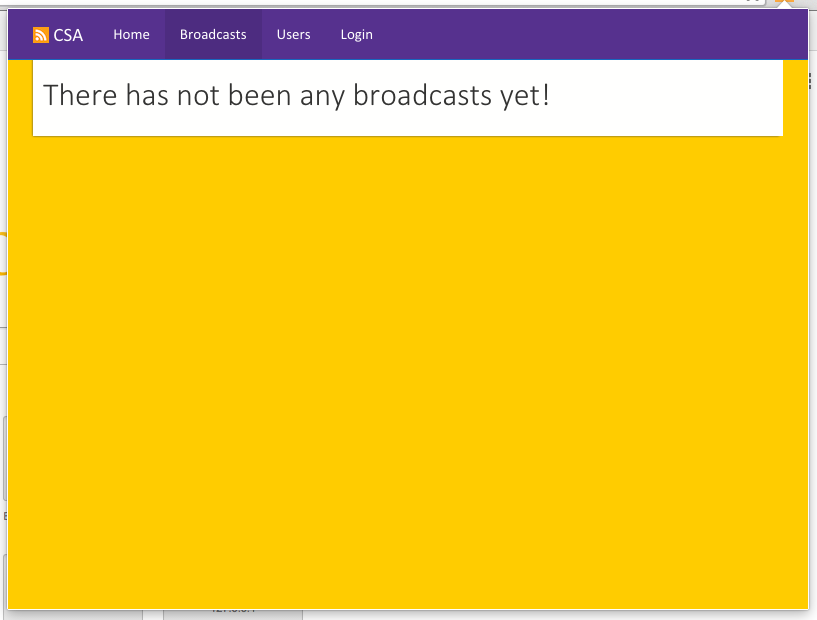
\includegraphics[width=0.8\textwidth]{bcpage}
\caption{Above we see the broadcasts screen with no broadcasts available.}
\end{figure}

\begin{figure}[!htbp]
\centering
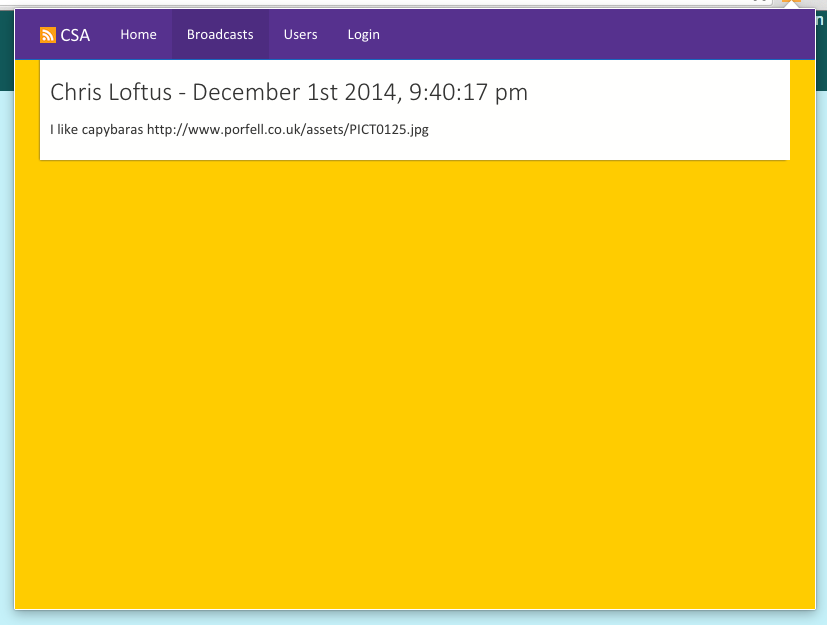
\includegraphics[width=0.8\textwidth]{populatebcpage}
\caption{This is what the populated broadcast screen looks like.}
\end{figure}

\begin{figure}[!htbp]
\centering
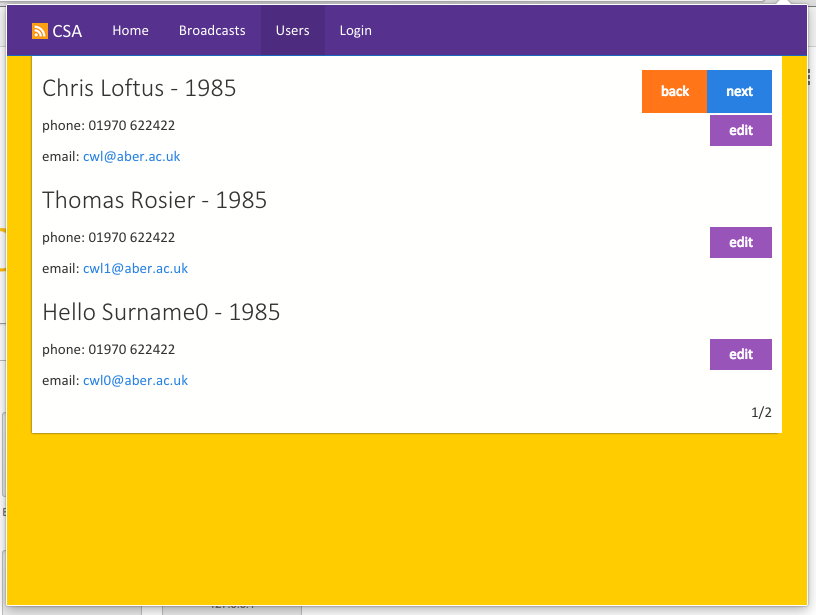
\includegraphics[width=0.8\textwidth]{userpage}
\caption{Here we have a screenshot of the user's screen.}
\end{figure}

\begin{figure}[!htbp]
\centering
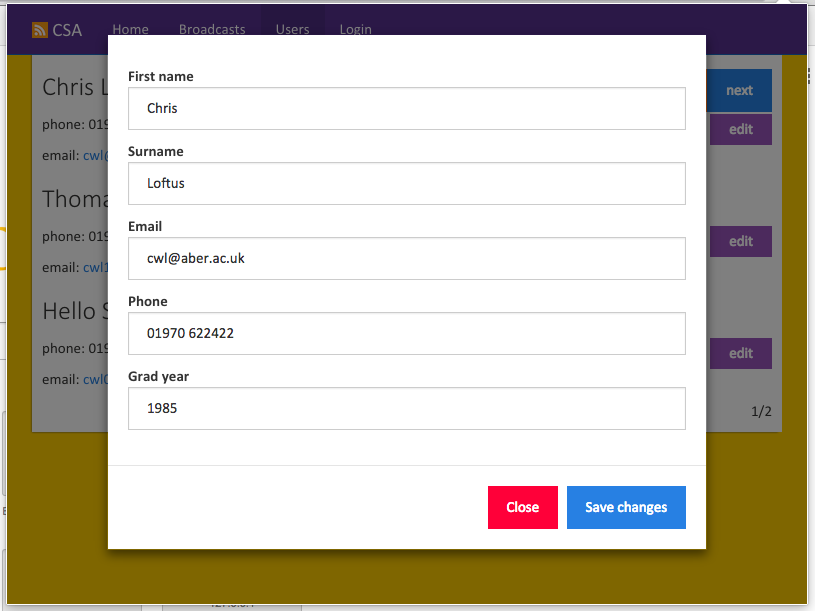
\includegraphics[width=0.8\textwidth]{modalpage}
\caption{Above we have a screenshot showing the appearance of the modal window we used to edit the user information.}
\end{figure}

\begin{figure}[!htbp]
\centering
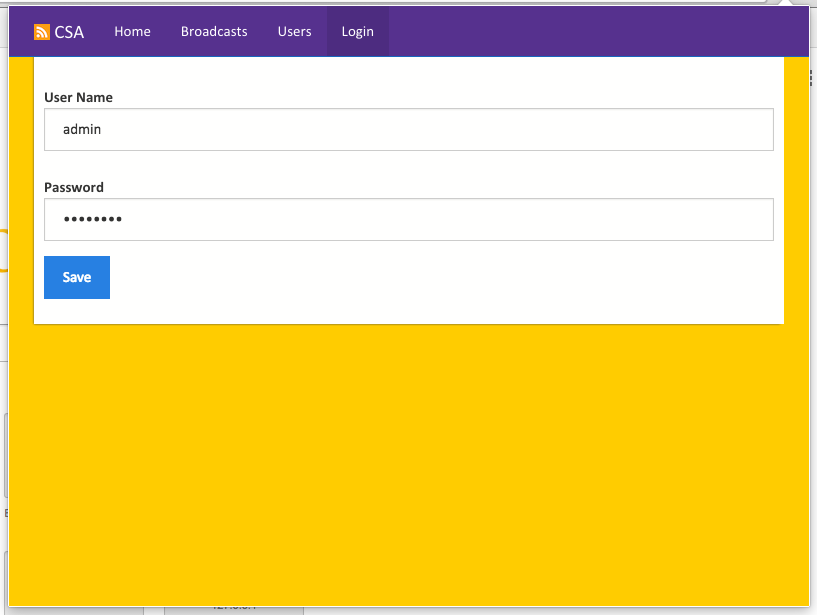
\includegraphics[width=0.8\textwidth]{loginpage}
\caption{This is a screenshot of the login screen.}
\end{figure}

\begin{figure}[!htbp]
\centering
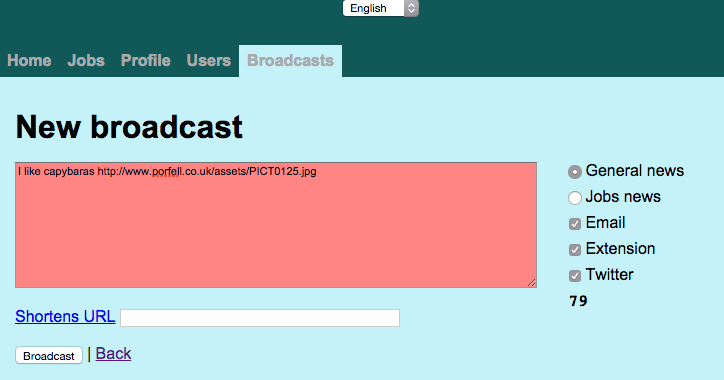
\includegraphics[width=0.75\textwidth]{createbc}
\caption{This is the unit tests for the background.js module for the browser extension.}
\end{figure}

\begin{figure}[!htbp]
\centering
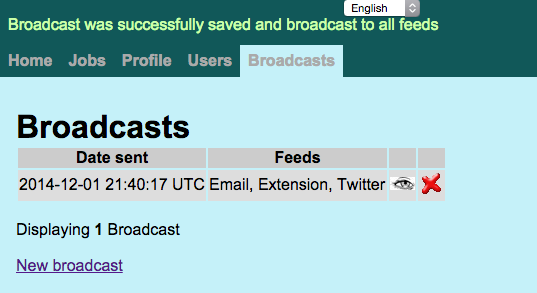
\includegraphics[width=0.75\textwidth]{confbc}
\caption{This is the unit tests for the background.js module for the browser extension.}
\end{figure}

\begin{figure}[!htbp]
\centering

\includegraphics[width=0.5\textwidth]{chromenotification}
\caption{This is the unit tests for the background.js module for the browser extension.}
\end{figure}

\begin{figure}[!htbp]
\centering

\includegraphics[width=0.5\textwidth]{operanotification}
\caption{This is the unit tests for the background.js module for the browser extension.}
\end{figure}

\begin{figure}[!htbp]
\centering
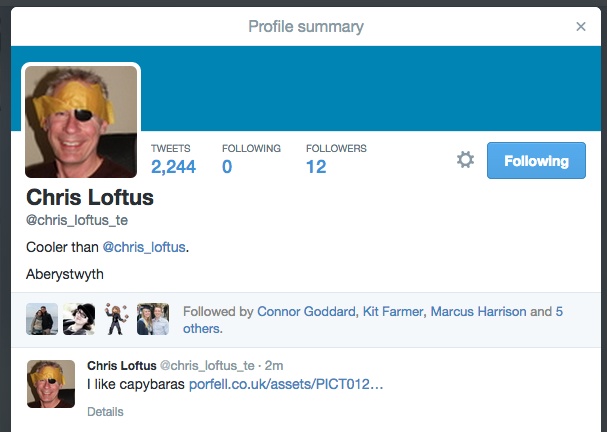
\includegraphics[width=0.8\textwidth]{twitterbc}
\caption{This is the unit tests for the background.js module for the browser extension.}
\end{figure}


\subsection{CS-Alumni Rails Application}

\subsubsection{New Additions}

\subsubsection{Modifications}


\subsection{Communication Between Applications}

\subsubsection{RESTful Web Interfaces}

\subsubsection{Data Flow Diagrams}


%-- Application Testing.
\section{Application Testing}

\subsection{QUnit Tests}



\begin{figure}[!htbp]
\centering
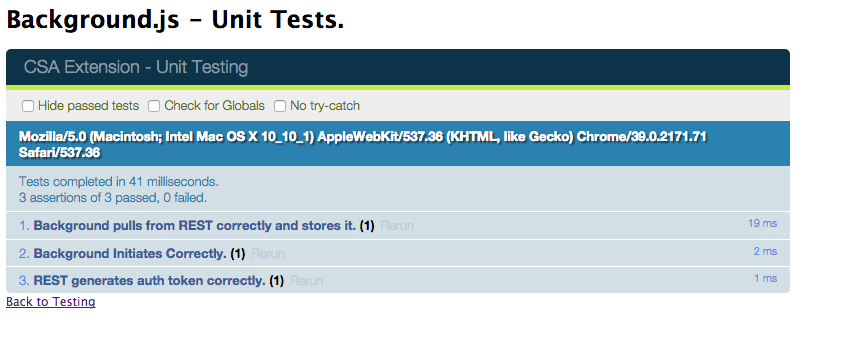
\includegraphics[width=\textwidth]{backgroundqunit}
\caption{This is the unit tests for the background.js module for the browser extension.}
\end{figure}

\begin{figure}[!htbp]
\centering
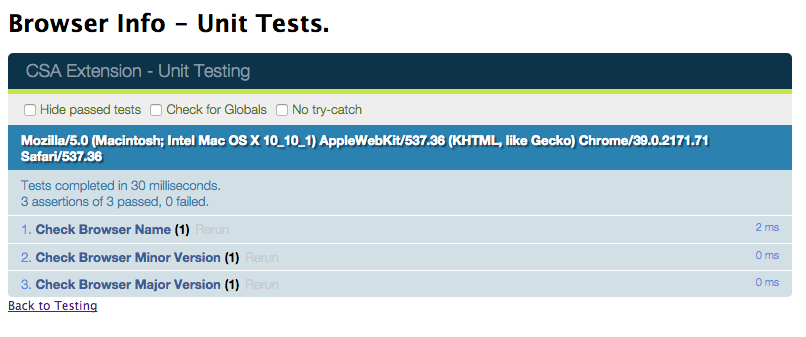
\includegraphics[width=\textwidth]{biqunit}
\caption{This images shows the browserinfo.js module completing its tests successfully.}
\end{figure}

\begin{figure}[!htbp]
\centering
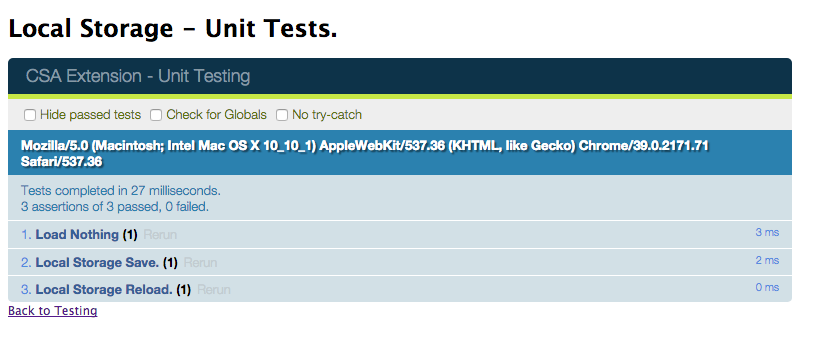
\includegraphics[width=\textwidth]{lsqunit}
\caption{This shows the LocalStorage.js module passing all its unit tests.}
\end{figure}

\begin{figure}[!htbp]
\centering
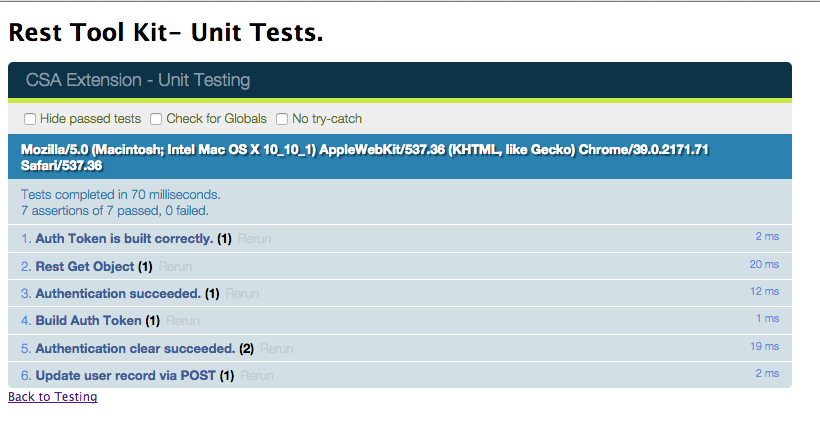
\includegraphics[width=\textwidth]{restqunit}
\caption{Above we see the RestToolKit.js module successfully completing all its unit tests.}
\end{figure}

\begin{figure}[!htbp]
\centering
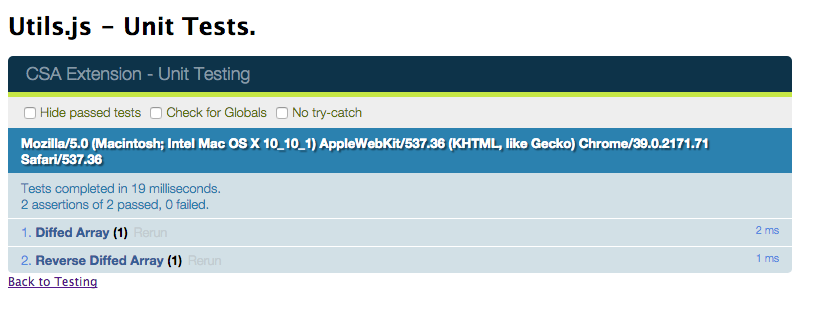
\includegraphics[width=\textwidth]{utilsqunit}
\caption{Included above we see the Utils.js module efficiently complete all of its unit tests.}
\end{figure}

%-- Technologies.
\section*{Technologies}

\subsection{CS-Alumni Rails Application}

\subsection{Communication Between Applications}


%-- Evaluation.
\section{Evaluation}

\section{Something Extra}
%-- Talk about pebble app here.
\begin{figure}[!htbp]
\centering
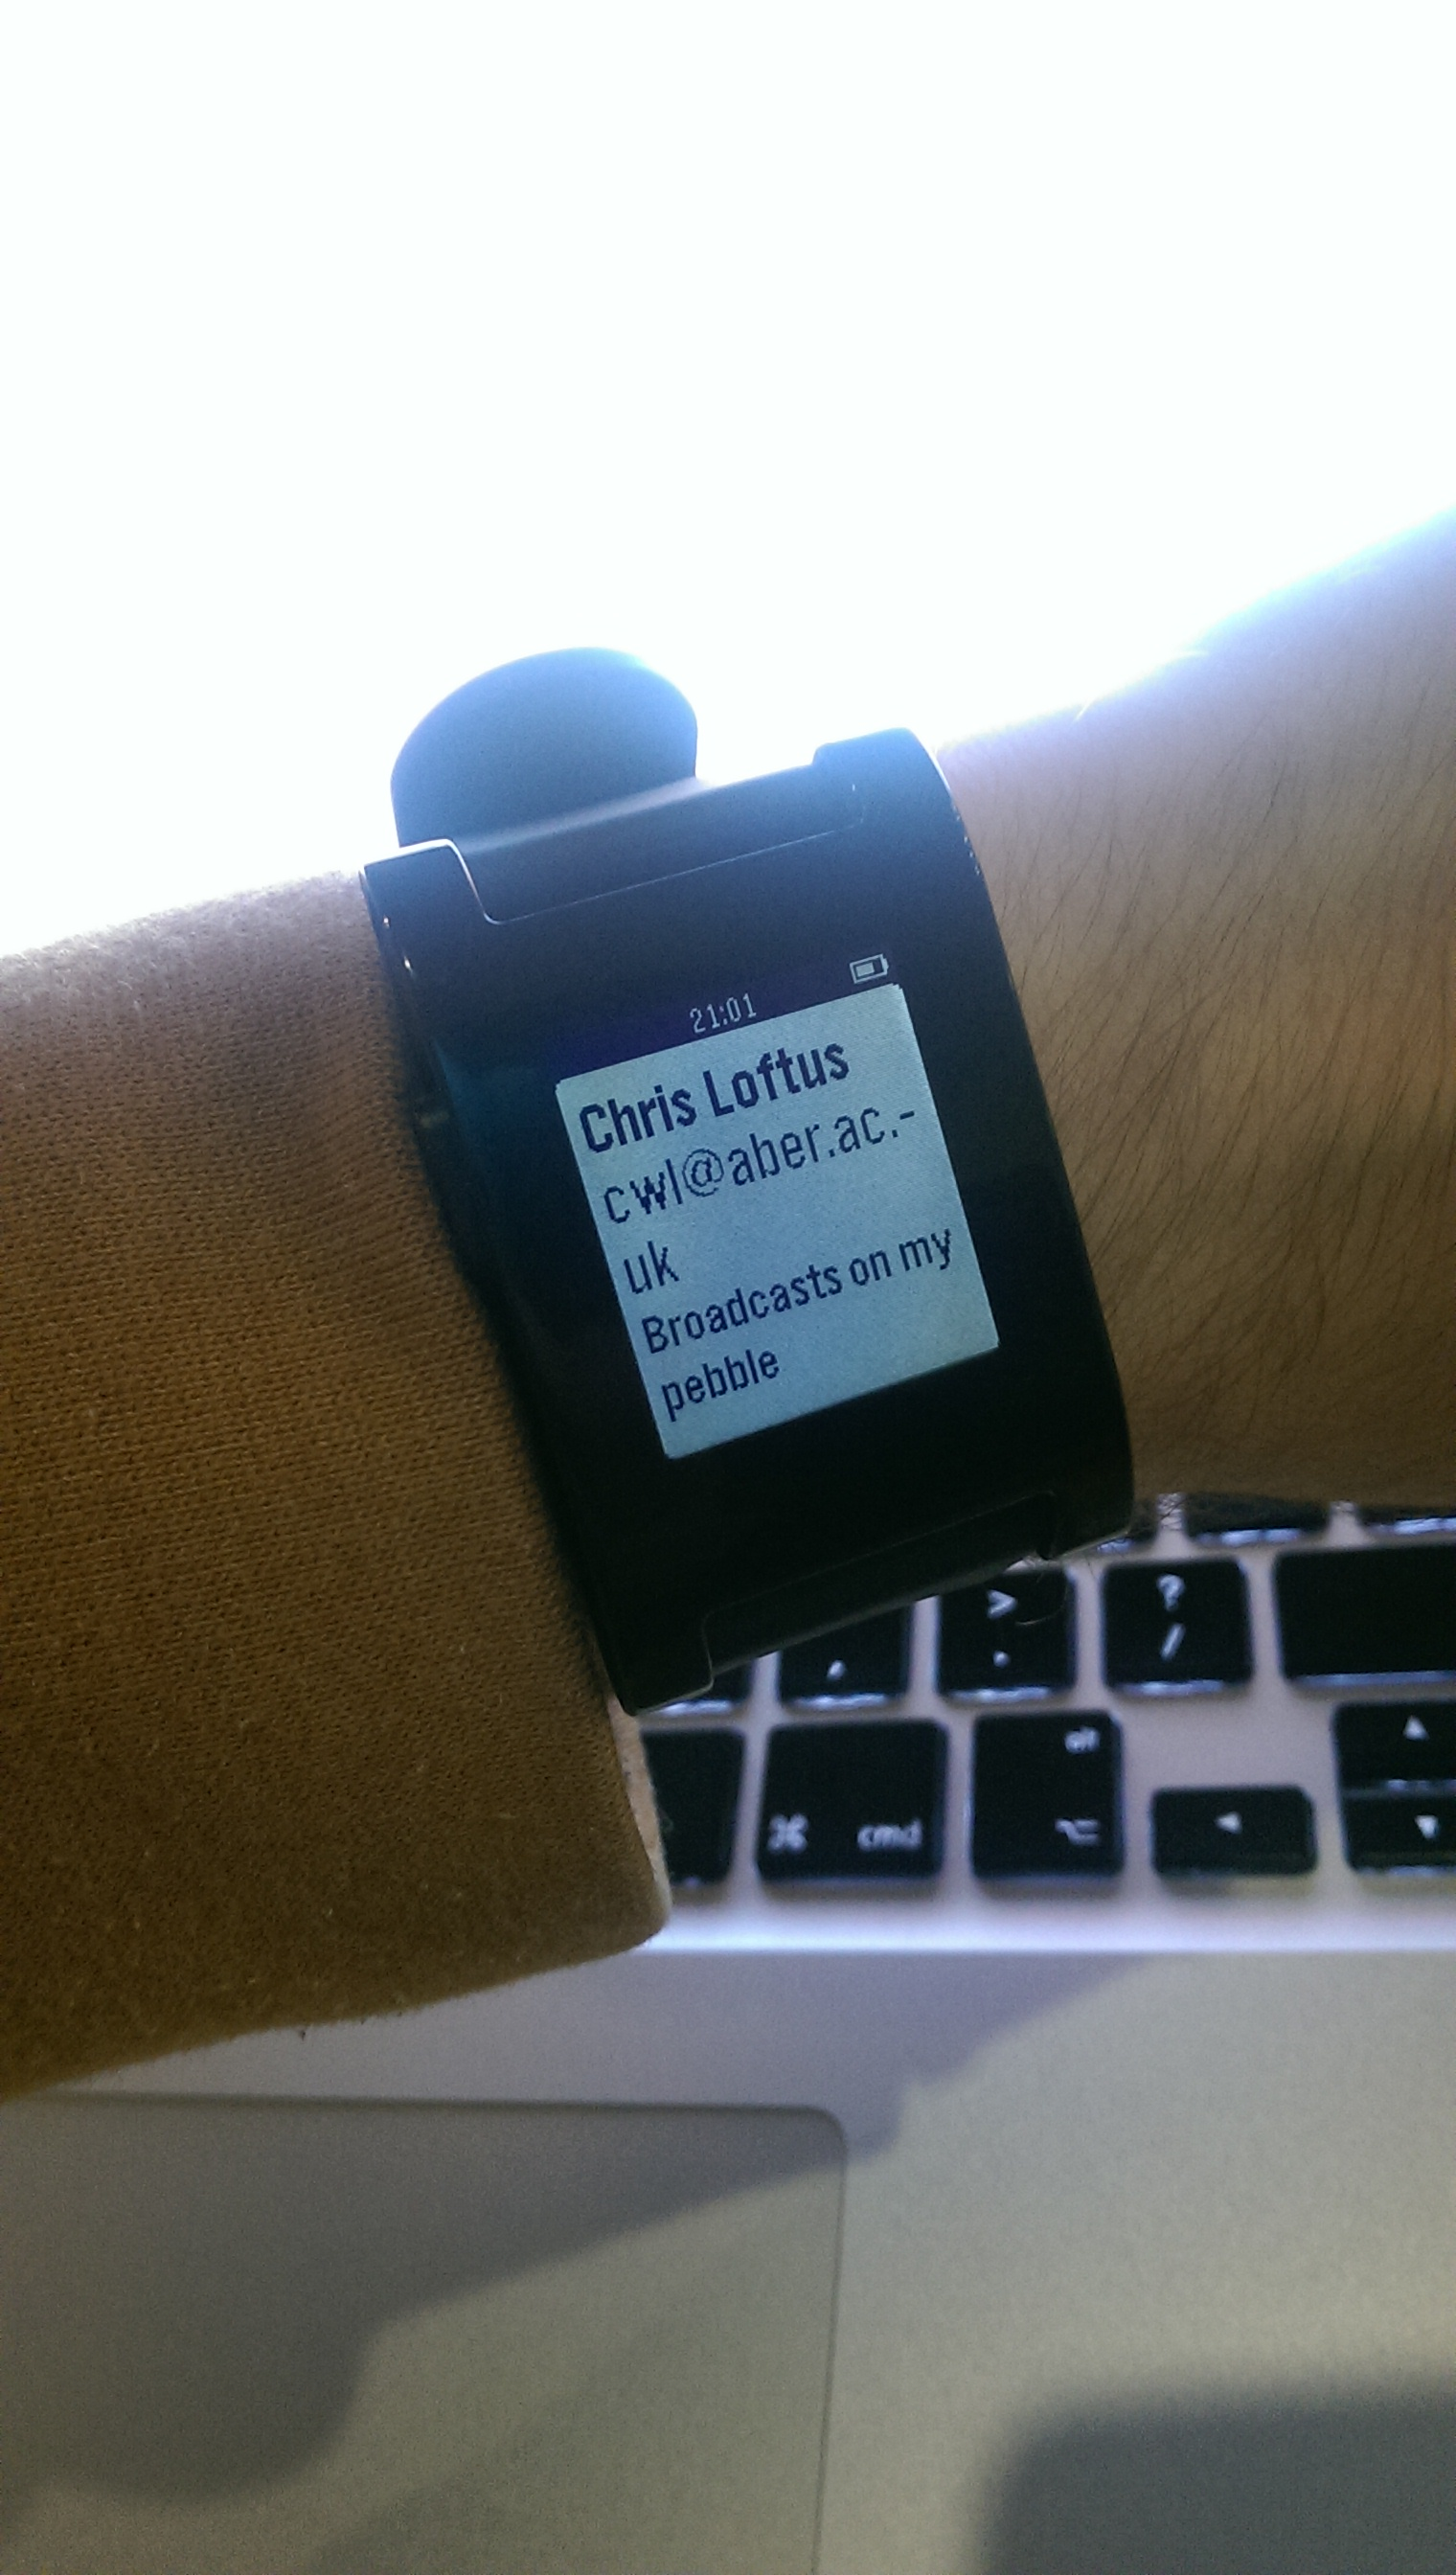
\includegraphics[width=0.5\textwidth]{pebble}
\caption{Above is a image of the Pebble smartwatch running the CSA application.}
\end{figure}

\begin{figure}[!htbp]
\centering
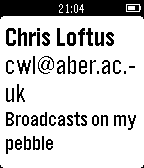
\includegraphics[width=0.25\textwidth]{pebblesh}
\caption{This is a screenshot taken from the Pebble smartwatch.}
\end{figure}

\newpage
%-- Attributions.
\section*{Attributions}

\newpage
\printbibliography

\end{document}